%#! platex main.tex

%======================================================================
\chapter{データ収集アプリケーションの設計・開発}

本研究の目的は, 食事中の音から食品を認識し, 咀嚼を検出することである. 本稿では, 機械学習技術を用いて食品認識と咀嚼検出を行うが, 機械学習モデルの訓練には, 大量のデータが必要とされるため, 必要なデータを効率的に収集するためのアプリケーションの開発が不可欠である. 食品認識と咀嚼検出には, 食事中の音データと食品ラベルと咀嚼タイムスタンプを含む正解データが必要である. 食事中の音を録音すること自体は, 例えばiPhoneのボイスメモのような一般的な録音アプリでも可能だが, 録音設定を固定にしないと分析精度に影響を及ぼす可能性がある. そのため, ノイズキャンセリングやサンプリングレートなどの録音設定を自由に調整できる機能が求められる. さらに, 咀嚼検出には咀嚼タイムスタンプの正解データが必要であるが, 食事中の動画や音声からこれらのデータを手作業でアノテーションするのは非常に困難である. これらのニーズはかなり特殊であり, 既存のアプリケーションではこれらのデータを効率的に収集するのは困難である. そのため, 研究の効率化のため, 図\ref{fig:application}に示すデータ収集アプリケーションを1から独自で開発した.また, TestFlight\footnote{TestFlight - Apple Developer~\url{https://developer.apple.com/testflight/}}を用いてiOSユーザ向けに配信できるようにし, 被験者自身の端末を用いて実験を行うことができるようにした.

\begin{figure}[t]
    \begin{center}
        \includegraphics[clip,  width=0.95\hsize]{img/application.png}
        \caption{データ収集アプリケーション}
        \label{fig:application}
    \end{center}
\end{figure}

今回開発したアプリは, 実験用のデータ収集アプリとしての要件を満たすために以下の機能が搭載されている. また, システム概要を図\ref{fig:application-abst}に示す.

\begin{figure}[t]
    \begin{center}
        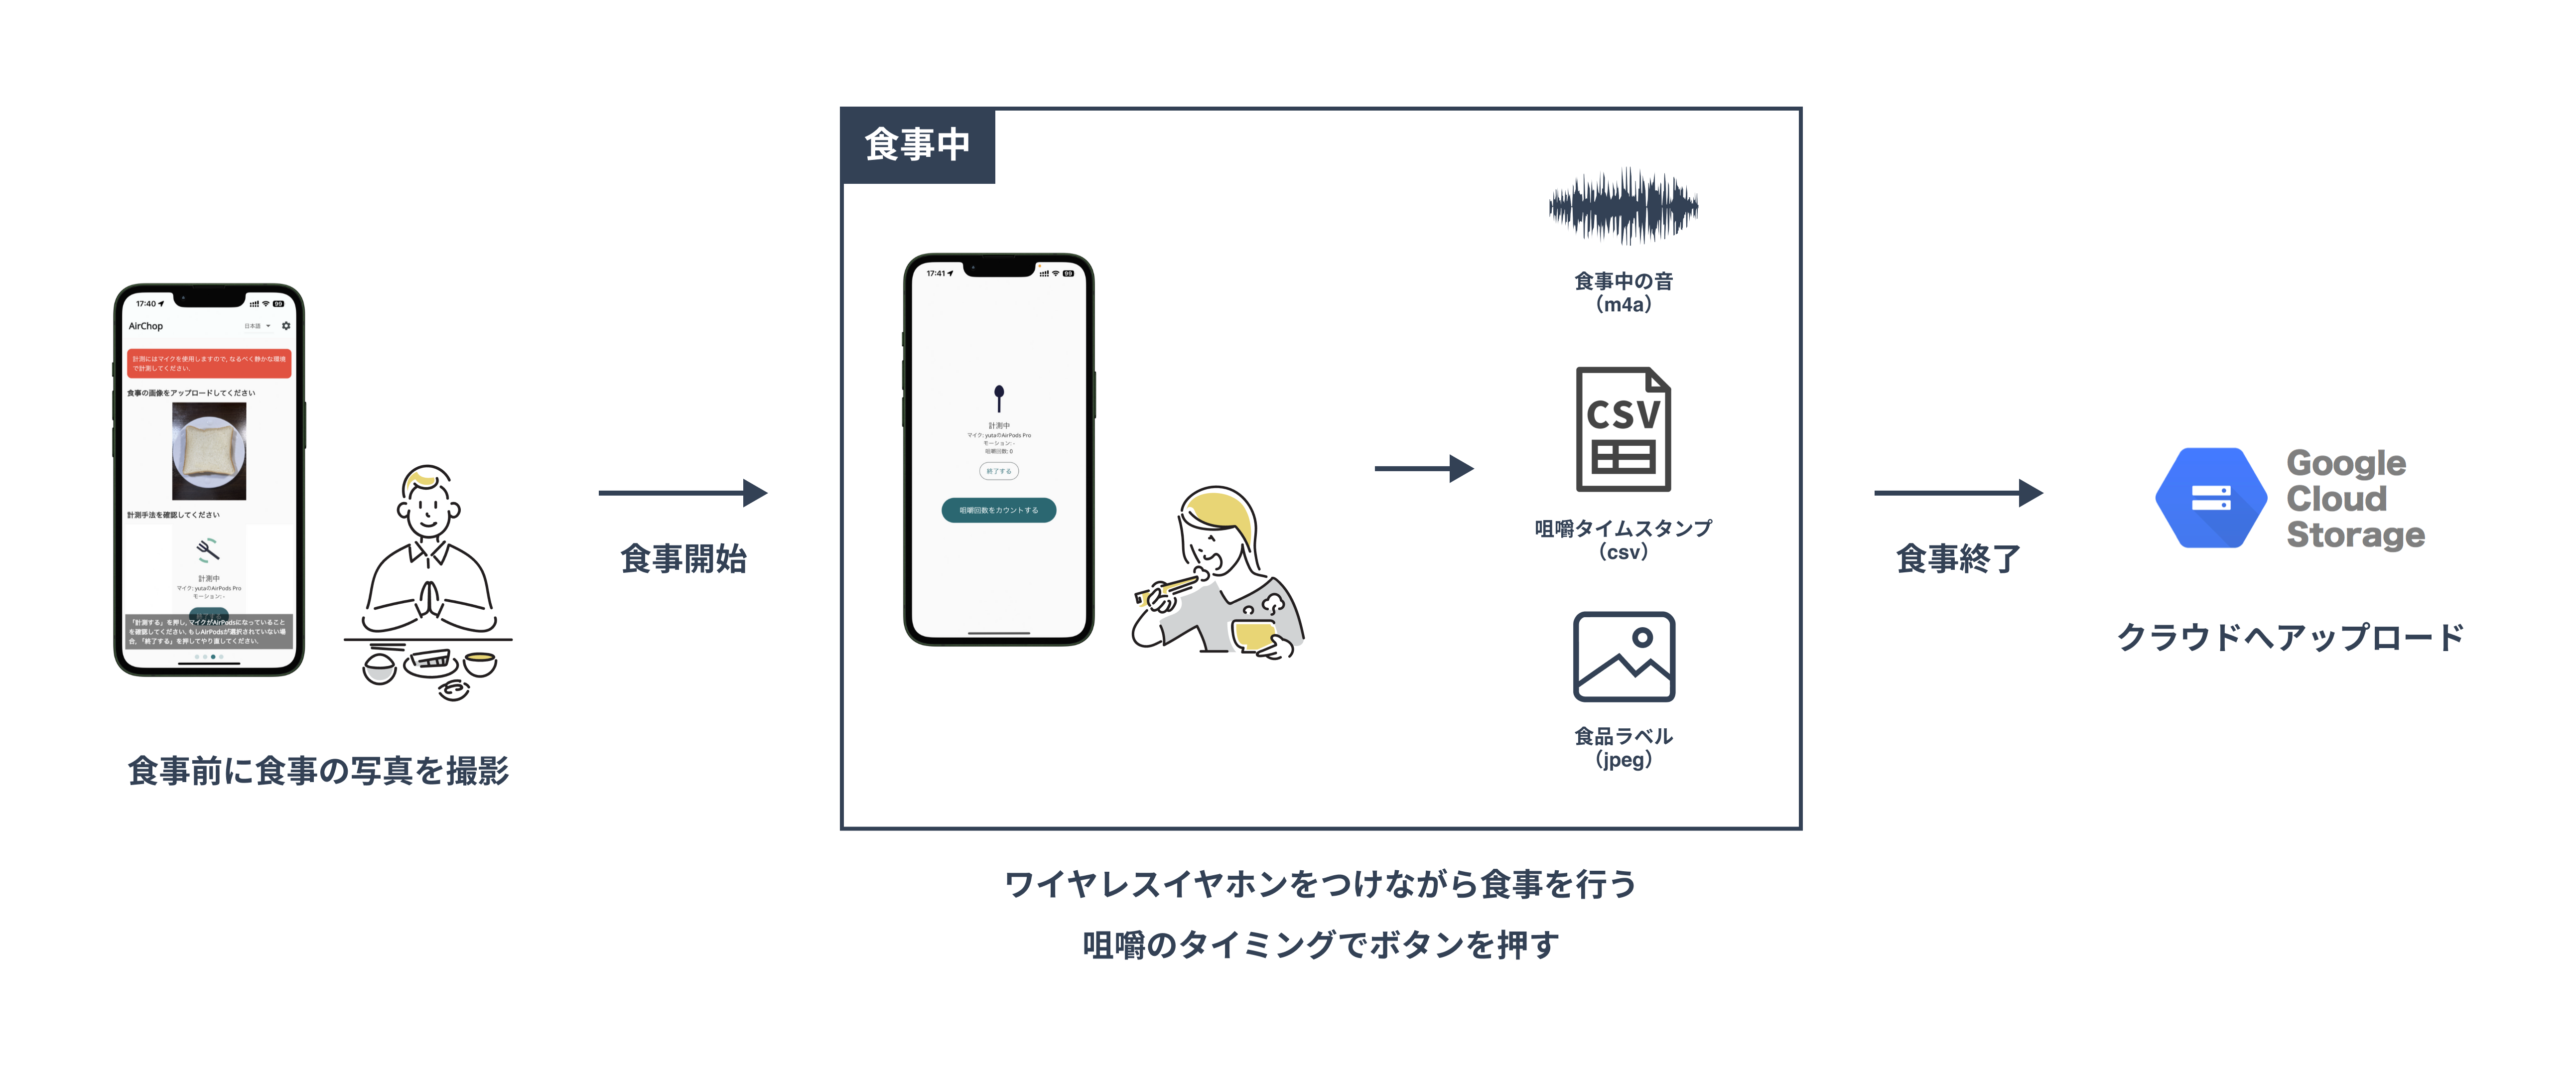
\includegraphics[clip,  width=0.95\hsize]{img/application-abst.png}
        \caption{データ収集アプリケーションのシステム概要}
        \label{fig:application-abst}
    \end{center}
\end{figure}

\begin{itemize}
    \item 食事中の音を録音する機能
    \item 咀嚼回数をアプリ利用者自身が計測する機能
    \item 実験時の食事を撮影する機能
    \item クラウドストレージにアップロードする機能
\end{itemize}

%----------------------------------------------------------------------
\section{食事中の音を録音する機能}

本稿では, ワイヤレスイヤホンに搭載されるマイクを用いて録音している. 食事中に発生する音は, 食べ物を噛む際に発生する咀嚼音, 皿や箸などのカトラリによる音, 環境ノイズを含む周囲の音から構成される. 食事中に発生する音の中でも, 特に咀嚼音が最も食事内容や咀嚼に関する情報を持っていると考えられるが, ワイヤレスイヤホンを用いた手法では, 咀嚼音が発生する口の近くに装着することができるため, より咀嚼音の要素を多く含んだ音を記録することができる.

録音機能の実装には, Apple社が提供するAVFAudio\footnote{AVFAudio | Apple Developer Documentation~\url{https://developer.apple.com/documentation/avfaudio}}を用いており, サンプリングレート・チャネル数・オーディオ品質・出力形式などを自由に設定することができる. オーディオ品質については, min・low・medium・high・maxの五段階あり, 品質の設定を上げるほど録音データの容量も大きくなる. また, ワイヤレスイヤホンでの録音を想定しているため, ワイヤレスイヤホンを接続していない場合は録音できないような仕様になっている. 今回使用したアプリケーションの録音の設定は以下の通りである.

\begin{itemize}
    \item サンプリングレート: 44100Hz
    \item チャネル数: 2
    \item オーディオ品質: high
    \item 出力形式: m4a
\end{itemize}

%----------------------------------------------------------------------
\section{咀嚼回数をアプリ利用者自身が計測する機能}

本稿では, 食事中の音から咀嚼回数の分析を行うためのアノテーション目的として, 咀嚼のタイミングを記録する機能を実装している. 図\ref{fig:application}に示すように, 計測開始後の画面上に咀嚼を記録するためのボタンが設置されており, 被験者には咀嚼を行ったタイミングでこのボタンを押下してもらう. 計測終了後に, 咀嚼タイミングのタイムスタンプをcsv形式で保存する.

\section{実験時の食事を撮影する機能}

録音データと咀嚼データがどの食事のデータであるかを対応づける目的として, 計測前に計測対象の食事の写真を撮影する機能を実装し, 画像データは録音データ・咀嚼データと対応づけが安易になるようファイル命名規則を決めて管理するようにした. 図\ref{fig:foods}に示す食事の画像は全てこのアプリケーションを通じて撮影されたものである.

\section{クラウドストレージにアップロードする機能}

データ収集を被験者自身の端末で行う想定なので, 本アプリケーションでは計測したデータをクラウド上に送信することでデータの管理を安易にした. クラウドのストレージサービスは, Google社が提供するCloud Storage\footnote{Cloud Storage | Google Cloud~\url{https://cloud.google.com/storage}}を採用した. 本アプリケーションでは, 録音を停止したタイミングで, 録音データ・咀嚼データ・食事画像データをCloud Storageにアップロードしている.

% 以下はRefTeX用
%%% Local Variables:
%%% mode: yatex
%%% TeX-master: "main"
%%% End:
